\documentclass[11pt, twocolumn]{article}
\usepackage{homework}
\usepackage{listings}
\usepackage[style=ieee]{biblatex}
\usepackage{mhchem}
\usepackage{hyperref}
\usepackage{subcaption}
\addbibresource{computing_report.bib}
\pagestyle{fancy}

% Change bibliography font size
\renewcommand*{\bibfont}{\footnotesize}

% Commands used for formatting heatmaps to the same height
\newdimen\imageheight
\settoheight{\imageheight}{
    \includegraphics[width=0.3325\textwidth,keepaspectratio]{asset/ibso_lambda_0.00_pro.png}
}

\newdimen\imageheightsecond
\settoheight{\imageheightsecond}{
    \includegraphics[width=0.3325\textwidth,keepaspectratio]{asset/ibso_eigenvalue_lambda_0.00_ret.png}
}

\definecolor{codegreen}{rgb}{0,0.6,0}
\definecolor{codegray}{rgb}{0.5,0.5,0.5}
\definecolor{codepurple}{rgb}{0.58,0,0.82}
\definecolor{backcolour}{rgb}{0.95,0.95,0.95}

\lstdefinestyle{mystyle}{
    backgroundcolor=\color{backcolour},   
    commentstyle=\color{codegreen},
    keywordstyle=\color{magenta},
    numberstyle=\tiny\color{codegray},
    stringstyle=\color{codepurple},
    basicstyle=\ttfamily\footnotesize,
    breakatwhitespace=false,         
    breaklines=true,                 
    captionpos=b,                    
    keepspaces=true,                 
    numbers=left,                    
    numbersep=5pt,                  
    showspaces=false,                
    showstringspaces=false,
    showtabs=false,                  
    tabsize=4
}

\lstset{style=mystyle}

% assignment information
\def\course{Vacation Placement}
\def\assignmentno{Local tidal tensor via ZAMO}
\def\assignmentname{Unified approach for stationary axisymmetric spacetime}
\def\name{EXET3567}
\def\time{\today}

\begin{document}


\begin{titlepage}
    \begin{center}
        \large
        \textbf{\course}

        \vfill

        \Huge
        \textbf{\assignmentno}

        \vspace{1.5cm}

        \large{\assignmentname}

        \vspace{3.5cm}

        % Additional information
        This report is submitted for replacement of practical work with a vacation placement.\\The placement was carried out under Department of Physics, University of Oxford.\\The placement took place from 12th August 2024 to 5th October 2024, 8 weeks in total.
        \vfill

        \large{EXET3567}

        \time
    \end{center}
\end{titlepage}


\twocolumn[
    \begin{@twocolumnfalse}
        \begin{abstract}
            We report the development of a suite of tools that numerically integrate the second-order geodesic equation and compute the local tidal tensor and its eigenvalues along the particle trajectory. Written in \texttt{C++}, the integrator admits an arbitrary stationary, axisymmetric spacetime metric and integrates the geodesic equations using an improved eighth-order Runge-Kutta method with adaptive step size. The flexibility of the approach is ensured by a \texttt{Mathematica} notebook that generates symbolic expressions for the metric, Christoffel symbols and the local tidal tensor. We present the workflow of this approach, discuss the design choices made for speed and accuracy and demonstrate its application to spherical spacetimes and the Kerr-Newman spacetime.
        \end{abstract}
        \vspace{1cm}
    \end{@twocolumnfalse}
]


%==========
\section{Introduction} \label{sec:intro}
%==========


Black holes (BHs) are generally surrounded by a population of stars in stable orbits. On rare occasions, a perturbation may cause a star to fall into a trajectory that leads it to the BH \cite{Mummery2023}. Due to the strong gravitational forces near the BH, it is possible that the tidal forces experienced by the star exceed its own self-gravitational forces, causing the star to disintegrate. This violent phenomenon, known as tidal disruption events (TDEs), produces bright electromagnetic signals that are hypothesised to reveal properties of the BH.

In recent years significant interest has been placed on the study of TDEs, partially because of the advent of better observational instruments that allow for more frequent detection of such events. Many theoretical studies have been carried out to understand the tidal forces experience by a star near a compact object like a BH. Such models allow us to predict when, where and how often a TDE may occur given the properties of the BH and the star, and thus allow inference to be made if a TDE is detected \cite{Mummery2023, Kesden2012}.

A large amount of work has been done in analysing tidal forces in various spacetime backgrounds. In his pioneering work, Marck \cite{Marck1983} derived the tidal tensor for a test particle in the Kerr spacetime using an ingenious tetrad formulation. However, the derivation includes a time-dependent dynamic angle (used to rotate two components of the tetrad) that makes it difficult to apply the results at an arbitrary location. Still, his work formed the basis of many subsequent studies, many of which only considered special locations where simplifications are possible.

Another set of studies\footnote{See accompanying \texttt{Mathematica} notebook and references therein.} investigated specific instances of spherical spacetimes that represent exotic solutions to Einstein's equations. These works constructed a tetrad suitable for radial geodesics ($\dot{\theta} = \dot{\phi} = 0$) and derived analytical expressions for the tidal tensor. However, while $\dot{\theta} = 0$ incurs no loss of generality due to spherical symmetry, setting $\dot{\phi} = 0$ is a strong and restrictive assumption: the test particle must have zero angular momentum. This is almost never the case for particles approaching a BH.

In light of the limits of current literature, we proposed a framework that allows for the computation of the local tidal tensor in a general stationary, axisymmetric spacetime in a recent work \cite{Anonymous2024}. The goal is to unify the results of previous studies and extend them to arbitrary locations in any stationary, axisymmetric spacetime. In this report, we describe the programmatic implementation of the theory and demonstrate its application to spherical spacetimes and the Kerr-Newman spacetime.

We use natural units where $G = c = 1$ and the signature $(-, +, +, +)$. Einstein's summation convention is assumed throughout.


%==========
\section{Theoretical Background} \label{sec:theory}
%==========


We briefly outline the theoretical background of our subsequent computational work. In general relativity, the geometry of spacetime is described by a metric tensor $g_{\mu\nu}$. The metric tensor can be viewed as a $4 \times 4$ symmetric matrix. In a stationary, axisymmetric spacetime, the metric tensor can be written in the form:
\begin{equation}
    g =
    \begin{pmatrix}
        g_{tt}    & g_{t\phi}    & 0                & 0            \\
        g_{t\phi} & g_{\phi\phi} & 0                & 0            \\
        0         & 0            & g_{\theta\theta} & 0            \\
        0         & 0            & 0                & g_{\phi\phi}
    \end{pmatrix} \, ,
\end{equation}
where the metric elements are functions of coordinates $r$ and $\theta$ only.


\subsection{Geodesic Motion}


In general, the equations of motion are given by the geodesic equation:
\begin{equation} \label{eq:geodesic}
    \frac{\mathrm{d}^2 x^{\mu}}{\mathrm{d}\tau^2} + \Gamma^{\mu}_{\nu\lambda} \frac{\mathrm{d} x^{\nu}}{\mathrm{d}\tau} \frac{\mathrm{d} x^{\lambda}}{\mathrm{d}\tau} = 0 \, ,
\end{equation}
where $\Gamma^{\mu}_{\nu\lambda}$ are the Christoffel symbols defined by:
\begin{equation}
    \Gamma^{\mu}_{\nu\lambda} = \frac{1}{2} g^{\mu\sigma} \left( \frac{\partial g_{\sigma\nu}}{\partial x^{\lambda}} + \frac{\partial g_{\sigma\lambda}}{\partial x^{\nu}} - \frac{\partial g_{\nu\lambda}}{\partial x^{\sigma}} \right) \, .
\end{equation}

Equation \eqref{eq:geodesic} are a set of coupled second-order differential equations that can be solved numerically to obtain the trajectory of a particle in a given spacetime once initial conditions are specified.


\subsection{Tidal Forces}


Tidal forces in general relativity are defined via the geodesic deviation equation:
\begin{equation}
    \frac{\mathrm{D}}{\mathrm{D} \tau^{2}} \delta x^{\mu} = R^{\mu}_{\alpha\nu\beta} U^{\alpha} U^{\beta} \delta x^{\nu} \, ,
\end{equation}
where $R^{\mu}_{\alpha\nu\beta}$ is the Riemann tensor and $U^{\mu} = \mathrm{d}x^{\mu}/\mathrm{d}\tau$ is the four-velocity of the particle.

This equation defines how two nearby geodesics, separated by $\delta x^{\mu}$, deviate further apart due to the curvature of spacetime. For a finite-size object, this defines the tidal forces. We define the tidal tensor as:
\begin{equation}
    C^{i}_{j} = -R^{i}_{\mu j \nu} U^{\mu} U^{\nu} \, .
\end{equation}

The tidal tensor is a $4 \times 4$ matrix that encodes the tidal forces experienced by a test particle, as measured by a distant observer. We need, however, the tidal forces experienced by the test particle in its local free falling (LFF) frame. The transformation of the tidal tensor between these frames is non-trivial and has only been done for spherical spacetimes \cite{Vandeev2022} and the Kerr spacetime \cite{Marck1983}. In a recent work \cite{Anonymous2024}, we developed a general approach to carry out this transformation for any stationary, axisymmetric spacetime by introducing an intermediate frame called the zero-angular-momentum observer (ZAMO) frame. In essence, we calculate the Riemann tensor in the distant observer frame and transform it to the ZAMO frame using the ZAMO tetrad. Then the ZAMO Riemann tensor is Lorentz boosted to the LFF frame to obtain the local tidal tensor. We invite the reader to consult this work for a detailed discussion of the theory.

The local tidal tensor $C^{\tilde{\mu}}_{\tilde{\nu}}$ is a  function of coordinates and velocities (in the distant observer frame), so we may evaluate this tensor and compute its eigenvalues and eigenvectors. A negative (positive) eigenvalue indicates a stretching (compressing) force along the corresponding eigenvector. Due to the definition of geodesic deviation, there is always a zero eigenvalue in the time direction \cite{Anonymous2024}.


%==========
\section{Symbolic Derivation} \label{sec:symbolic}
%==========


From the previous section, we identify two important algebraic objects that are essential for computation but virtually impossible to derive by hand: the Christoffel symbols $\Gamma^{\mu}_{\nu\lambda}$ and the local tidal tensor $C^{\tilde{\mu}}_{\tilde{\nu}}$. We describe below how we derive these objects symbolically using \texttt{Mathematica}.


\subsection{Christoffel Symbols}


The Christoffel symbols are a collection of partial derivatives of the metric tensor. In some previous work \cite{Abdikamalov2019} that involved relativistic ray-tracing in a general spacetime, this is done with numerical differentiation. However, this not only introduces numerical errors but is also computationally expensive since the Christoffel symbols are needed at every step of the integration. It is also cumbersome to construct a script that carries out the differentiation at runtime for an arbitrary metric.

The power of a computer algebra system like \texttt{Mathematica} shines here. \texttt{Mathematica}'s powerful symbolic manipulation capabilities allow us to derive the Christoffel symbols given an arbitrary metric tensor. A \texttt{Mathematica} notebook is used to implement the definition of $\Gamma^{\mu}_{\nu\lambda}$ to output their exact expressions. Elements of $\Gamma^{\mu}_{\nu\lambda}$ are convoluted functions of the coordinates $r$ and $\theta$ that are impossible to track by hand. We hence export these expressions to a \texttt{C++} function that can be called by the integrator at each iteration.


\subsection{Tidal Tensor}


We may also implement the algorithm in \texttt{Mathematica} using its tensor manipulation capabilities. The algorithm eventually yields a local tidal tensor $C^{\tilde{\mu}}_{\tilde{\nu}}$ that contains extremely complicated expressions that cannot be simplified in most situations.

Nevertheless, these expressions are functions of the coordinates and the velocities of the test particle. There are two ways of using the tidal tensor. If the first integrals of the geodesic equations are known, we can replace the velocities with expressions of the coordinates. This may allow for simplification of the tidal tensor in some special cases, such as spherical spacetimes. If the first integrals are not used, we may numerically integrate the geodesic equations and compute the evolution of the tidal tensor along the trajectory. This is achieved by outputting the symbolic expressions of the tidal tensor to a \texttt{C++} function that is called by the integrator after the geodesic equations are solved at each step.


%==========
\section{Numerical Computation} \label{sec:numerical}
%==========


We now describe the design and implementation of the numerical integrator. We note that the tidal tensor is in general a sensitive function of the coordinates and velocities of the test particle. The usual RK45 method suffices in giving somewhat accurate tidal eigenvalues, but the eigenvectors are not reliable. We hence opt for an eighth-order Dormand-Prince (DOP853) method described in \cite{Press2007}. DOP853 is an eighth-order Runge-Kutta method with twelve evaluations. This approach is more computationally expensive but provides a more reliable evolution of the tidal tensor along the trajectory. Here we briefly describe the procedure of the algorithm.


\subsection{Dormand-Prince Algorithm}


We attempt to solve the full second-order geodesic equation \eqref{eq:geodesic} using a Runge-Kutta method. Let us define the state vector $y$ as:
\begin{equation}
    y = (t, r, \theta, \phi, \dot{t}, \dot{r}, \dot{\theta}, \dot{\phi})^{\intercal} \, .
\end{equation}

The derivative of the state vector is defined by the geodesic equation:
\begin{equation}
    \frac{\mathrm{d}y}{\mathrm{d}\tau} = \mathbf{A}(y) =
    \begin{pmatrix}
        \dot{t}                                               \\
        \dot{r}                                               \\
        \dot{\theta}                                          \\
        \dot{\phi}                                            \\
        -\Gamma^{t}_{\mu\nu} \dot{x}^{\mu} \dot{x}^{\nu}      \\
        -\Gamma^{r}_{\mu\nu} \dot{x}^{\mu} \dot{x}^{\nu}      \\
        -\Gamma^{\theta}_{\mu\nu} \dot{x}^{\mu} \dot{x}^{\nu} \\
        -\Gamma^{\phi}_{\mu\nu} \dot{x}^{\mu} \dot{x}^{\nu}
    \end{pmatrix} \, .
\end{equation}

The general form of an eighth-order Runge-Kutta method with twelve evaluations is given by:
\begin{equation}
    \begin{split}
        k_{i} &= h \mathbf{A} \left( y + \sum_{j=1}^{i-1} a_{ij} k_{j} \right) \, , \\
        y_{n+1} &= y_{n} + \sum_{i=1}^{12} b_{i} k_{i} \, .
    \end{split}
\end{equation}
where $h$ is the step size and $a_{ij}$, $b_{i}$ are coefficients that define the method.


\subsection{Adaptive Step Size Control}


In order to implement an adaptive step size control, we need to give an estimate of the error made at each step. This is realised by evaluating what is know as the embedded formula $y_{n+1}^{*}$. The embedded function should be some different linear combination of $k_{i}$ that is of a lower order than $y_{n+1}$. The authors of DOP853 proposed two embedded formulae of orders six and four:
\begin{equation}
    \begin{split}
        y_{n+1}^{(5)} &= y_{n} + \sum_{i=1}^{7} \hat{b}_{i} k_{i} + \mathcal{O}(h^{6}) \, , \\
        y_{n+1}^{(3)} &= y_{n} + \sum_{i=1}^{7} \tilde{b}_{i} k_{i} + \mathcal{O}(h^{4}) \, ,
    \end{split}
\end{equation}
so that we can define two vectors of errors:
\begin{equation}
    \begin{split}
        \epsilon_{5} &= y_{n+1}^{(5)} - y_{n+1} = \mathcal{O}(h^{6}) \, , \\
        \epsilon_{3} &= y_{n+1}^{(3)} - y_{n+1} = \mathcal{O}(h^{4}) \, .
    \end{split}
\end{equation}

For each of the error vectors, we define a scalar error estimate using the Euclidean norm:
\begin{equation}
    \text{err} = \sqrt{\frac{1}{N} \sum_{i=1}^{N} \left[ \frac{\epsilon_{(i)}}{\text{scale}_{(i)}} \right]^{2}} \, ,
\end{equation}
where we define the scaling vector as:
\begin{equation}
    \text{scale} = \text{tol} + \text{tol} \times \max(|y_{n}|, |y_{n+1}|) \, ,
\end{equation}
where $\text{tol}$ is some small user-defined tolerance.

We finally define the actual error estimate as:
\begin{equation}
    \text{err} = \text{err}_{5} \frac{\text{err}_{5}}{\sqrt{\text{err}_{5}^{2} + 0.01 \times \text{err}_{3}^{2}}}\, .
\end{equation}

The choice of this error estimate is such that if $\text{err}_{5} \ll \text{err}_{3}$, this gives an $\mathcal{O}(h^{8})$ error estimate. If $\text{err}_{5}$ for some reason becomes large or $\text{err}_{3}$ becomes small, $\text{err}$ still gives a reasonable basis for step size control \cite{Press2007}. In practice, this method proves more robust than taking a simple eighth-order error estimate.

Given the error estimate, we may adjust the step size for the next iteration using the formula:
\begin{equation}
    h_{\text{next}} = S \times h \left( \frac{1}{\text{err}} \right)^{1/8} \, ,
\end{equation}
where $S=0.95$ is a safety factor that ensures the step size does not change too drastically.

Invariant quantities such as energy and angular momentum serve as a check for the accuracy of the integrator. After each step, we evaluate these quantities and ensure that they are not different from their initial values by more than some small tolerance.

\subsection{Variable Substitution}


We note that a metric and thus the Christoffel symbols generally contain trigonometric functions of $\theta$ that are computationally expensive to evaluate. Hence, in all of the above computations, we introduce $\chi \equiv \cos{\theta}$ as a substitution that changes all trigonometric functions to algebraic ones. The substitution is done in \texttt{Mathematica} before generating the symbolic expressions. In practice, this significantly speeds up the \texttt{C++} computation by almost $50\%$.


%==========
\section{Spherical Spacetimes} \label{sec:spherical}
%==========


While the ZAMO transformation yields complicated expressions for the tidal tensor, it turns out to be possible to derive the local tidal tensor for a general spherical spacetime, given by the metric:
\begin{equation}
    \begin{split}
        g_{tt} &= -A(r) \, , \qquad g_{rr} = B(r) \, , \\
        g_{\theta\theta} &= r^{2} \, , \qquad g_{\phi\phi} = r^{2} \sin^{2}{\theta} \, .
    \end{split}
    \label{eq:spherical_metric}
\end{equation}

The resulting expressions of the local tidal tensor, presented in the Appendix, are lengthy but tractable by hand. This means that the problem of local tidal tensor can be fully solved for any spherical spacetime, encompassing a wide range of previous works.

Specific instances of $A(r)$ and $B(r)$ may be substituted and checked against the literature. Consider, for example, the Reissner-Nordstr\"{o}m (RN) spacetime with $A(r) = 1 - 2M/r + Q^{2}/r^{2}$ and $B(r) = 1/A(r)$. The tidal tensor has the eigenvalues:
\begin{equation}
    \begin{split}
        \lambda_{1} &= \frac{r^{3} - Q^{2} r^{2}}{r^{6}} \, , \\
        \lambda_{2} &= \frac{-2r^{3} + 3Q^{2} r^{2} - 3l_{z}^{2} r + 4Q^{2}l_{z}^{2}}{r^{6}} \, , \\
        \lambda_{3} &= \frac{r^{3} - Q^{2} r^{2} + 3l_{z}^{2} r - 2Q^{2}l_{z}^{2}}{r^{6}} \, .
    \end{split}
\end{equation}

Setting $l_{z} = 0$ gives the results in \cite{Crispino2016} which only studied radial geodesics. Further setting $Q = 0$ gives the well-known Schwarzschild results.


%==========
\section{Kerr-Newman Spacetime} \label{sec:kn}
%==========


We now demonstrate the application of the integrator to the Kerr-Newman (KN) spacetime, the most general black hole solution to Einstein's equations. The KN metric describes the spacetime geometry around a rotating, charged black hole:
\begin{equation}
    \begin{split}
        g_{tt} &= -\frac{\Delta - a^{2} \sin^{2}{\theta}}{\Sigma} \, , \\
        g_{rr} &= \frac{\Sigma}{\Delta} \, , \\
        g_{\theta\theta} &= \Sigma \, , \\
        g_{\phi\phi} &= \frac{(r^{2} + a^{2})^{2} - \Delta a^{2} \sin^{2}{\theta}}{\Sigma \sin^{2}{\theta}} \, , \\
        g_{t\phi} &= -\frac{2 a r \sin^{2}{\theta}}{\Sigma} \, ,
    \end{split}
\end{equation}
where:
\begin{equation}
    \begin{split}
        \Delta &\equiv r^{2} - 2r + a^{2} + Q^{2} \, , \\
        \Sigma &\equiv r^{2} + a^{2} \cos^{2}{\theta} \, .
    \end{split}
\end{equation}
where $a$ and $Q$ are measures of the angular momentum and charge of the black hole respectively and we have set the mass of the black hole to unity.

Note that a horizon exists at $r_{\pm} = 1 \pm \sqrt{1 - a^{2} - Q^{2}}$. This also means that $a^{2} + Q^{2} \leq 1$ to prevent a naked singularity, a case not considered here but discussed in \cite{Anonymous2024}.

By choosing suitable initial conditions and conserved quantities, we may set a massive particle on a special class of geodesics called the innermost bound spherical orbits (IBSOs). These orbits are special because they represent the closest approach to a black hole without falling into the event horizon. IBSOs constitute a \textit{separatrix} between plunging orbits and escaping orbits and they give the most extreme tidal forces experienced by a test particle \cite{Mummery2023}. In Figure \ref{fig:ibso}, we show the three-dimensional plot of a sample IBSO in the KN spacetime. Note how the particle starts from a parabolic flyby and asymptotically approaches a constant radial distance.

\begin{figure}[ht!]
    \centering
    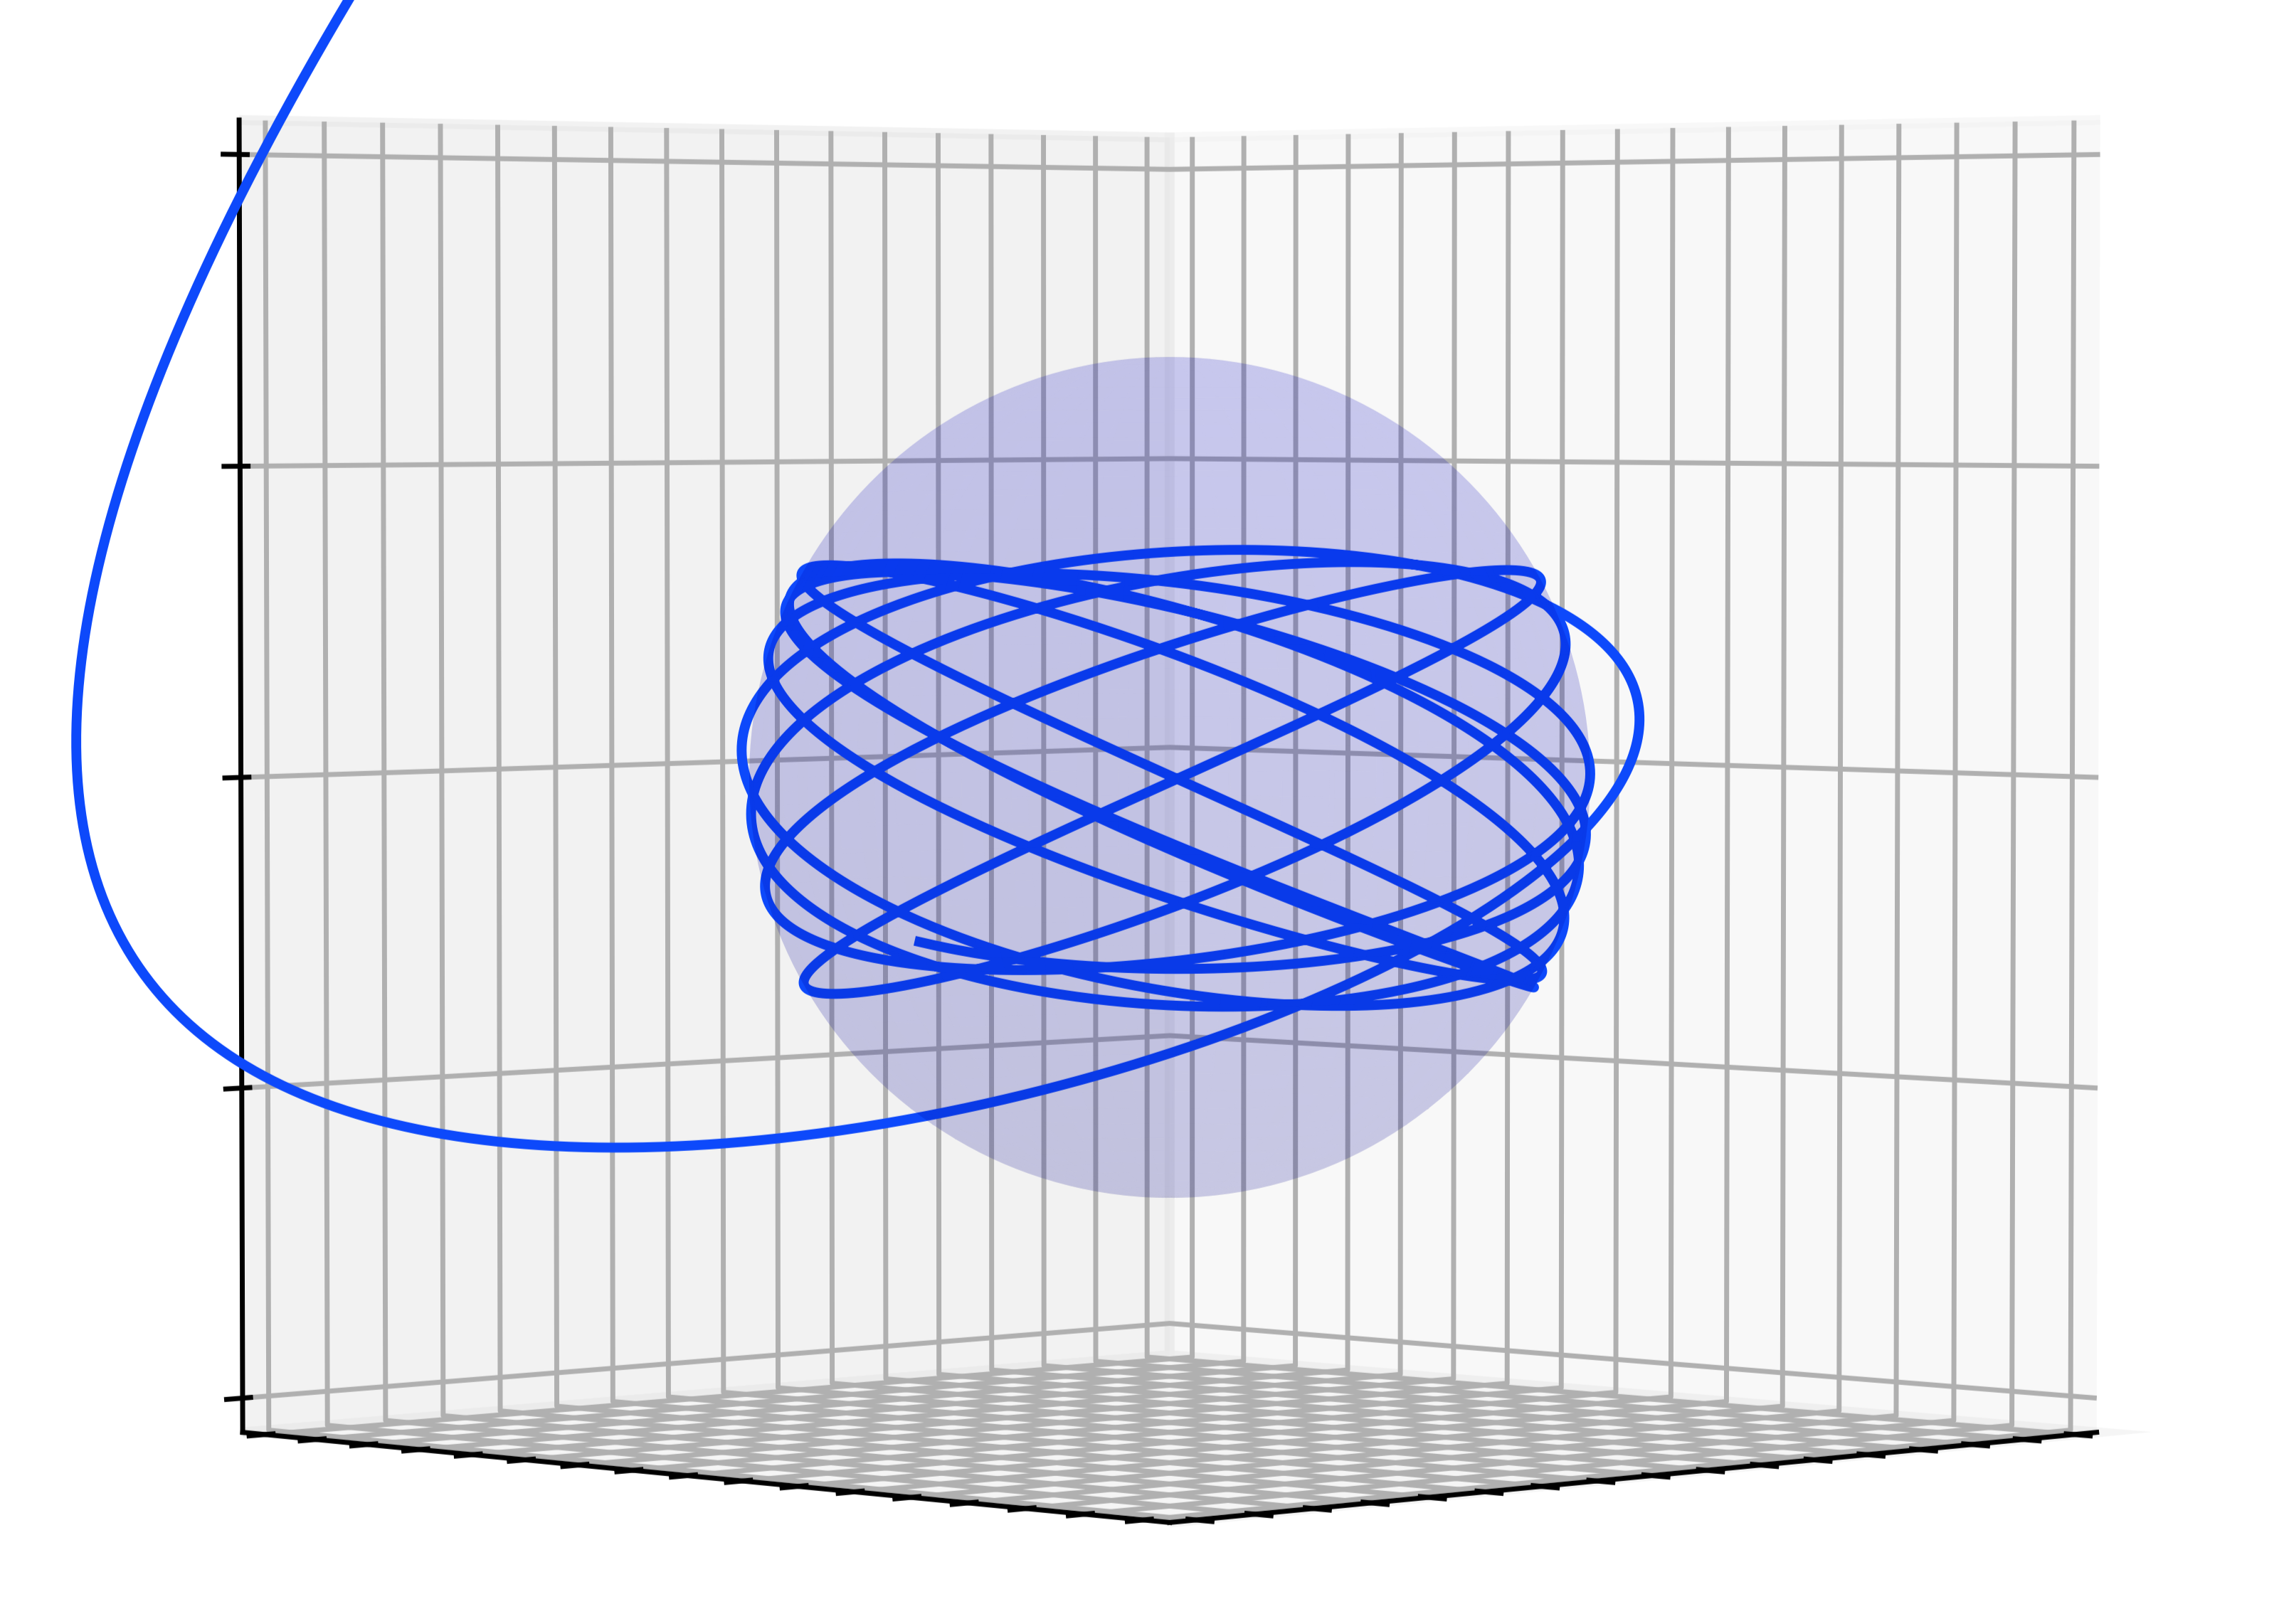
\includegraphics[width=\columnwidth]{asset/IBSO_3D_a_0.50_Q_0.50_lambda_0.50.png}
    \caption{IBSO in Kerr-Newman spacetime with $a = 0.5$, $Q = 0.5$, $\Lambda = 0.5$, $r_{\text{IBSO}} \approx 2.7014$.}
    \label{fig:ibso}
\end{figure}

In Figure \ref{fig:kn_simulations}, we show the evolution of the tidal eigenvalues along prograde three sample IBSO geodesics. Observe that the radial distance approaches a constant value, indicating that the particle reaches a spherical orbit asymptotically. Note that the (non-zero) eigenvalues are strong functions of both $r$ and $\theta$. Maximum tidal forces are experienced at the equatorial plane $\theta = \pi/2$ where the effect of spin is most pronounced. Increasing $a$ or $Q$ increases the maximum tidal forces experienced by the particle. This is mainly because higher $a$ or $Q$ allows a smaller IBSO radius where spacetime curvature is more extreme.

\begin{figure}[ht!]
    \centering
    \begin{subfigure}[b]{\columnwidth}
        \centering
        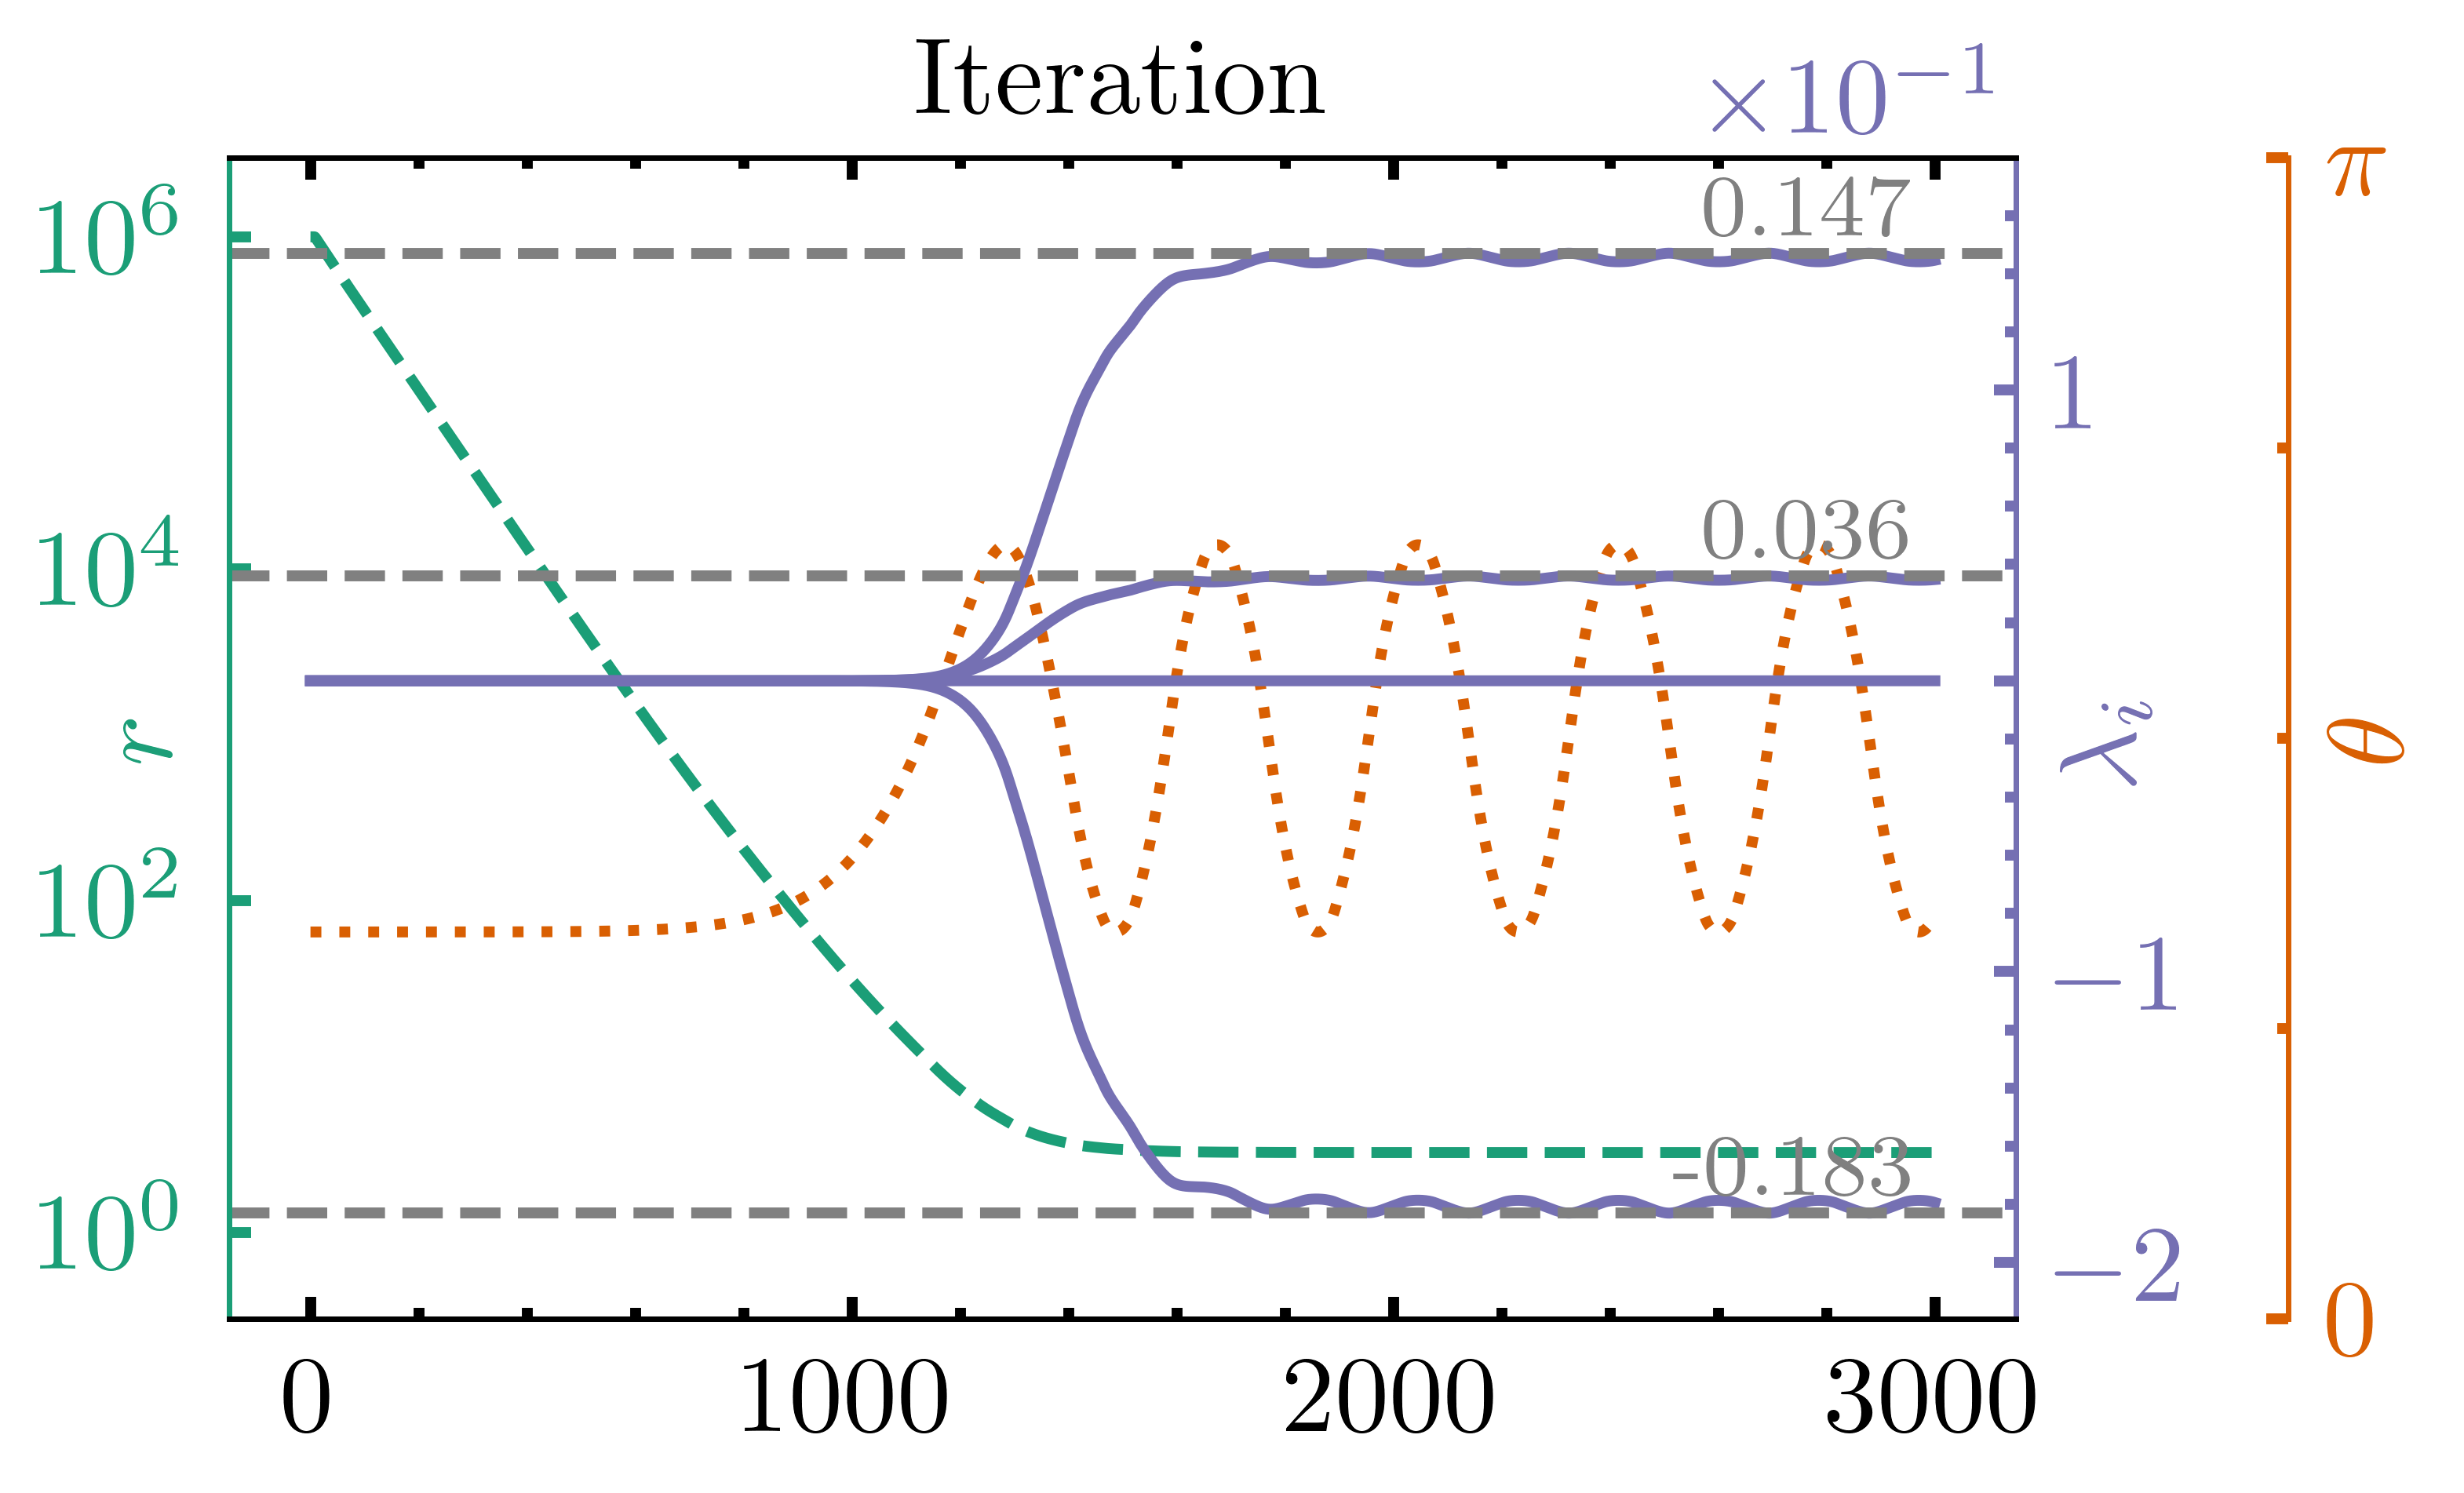
\includegraphics[width=\textwidth]{asset/eigensystem_a_0.50_Q_0.00_lambda_0.50_pro.png}
        \caption{$\Lambda = 0.5$, $a = 0.5$, $Q = 0$}
    \end{subfigure}
    \begin{subfigure}[b]{\columnwidth}
        \centering
        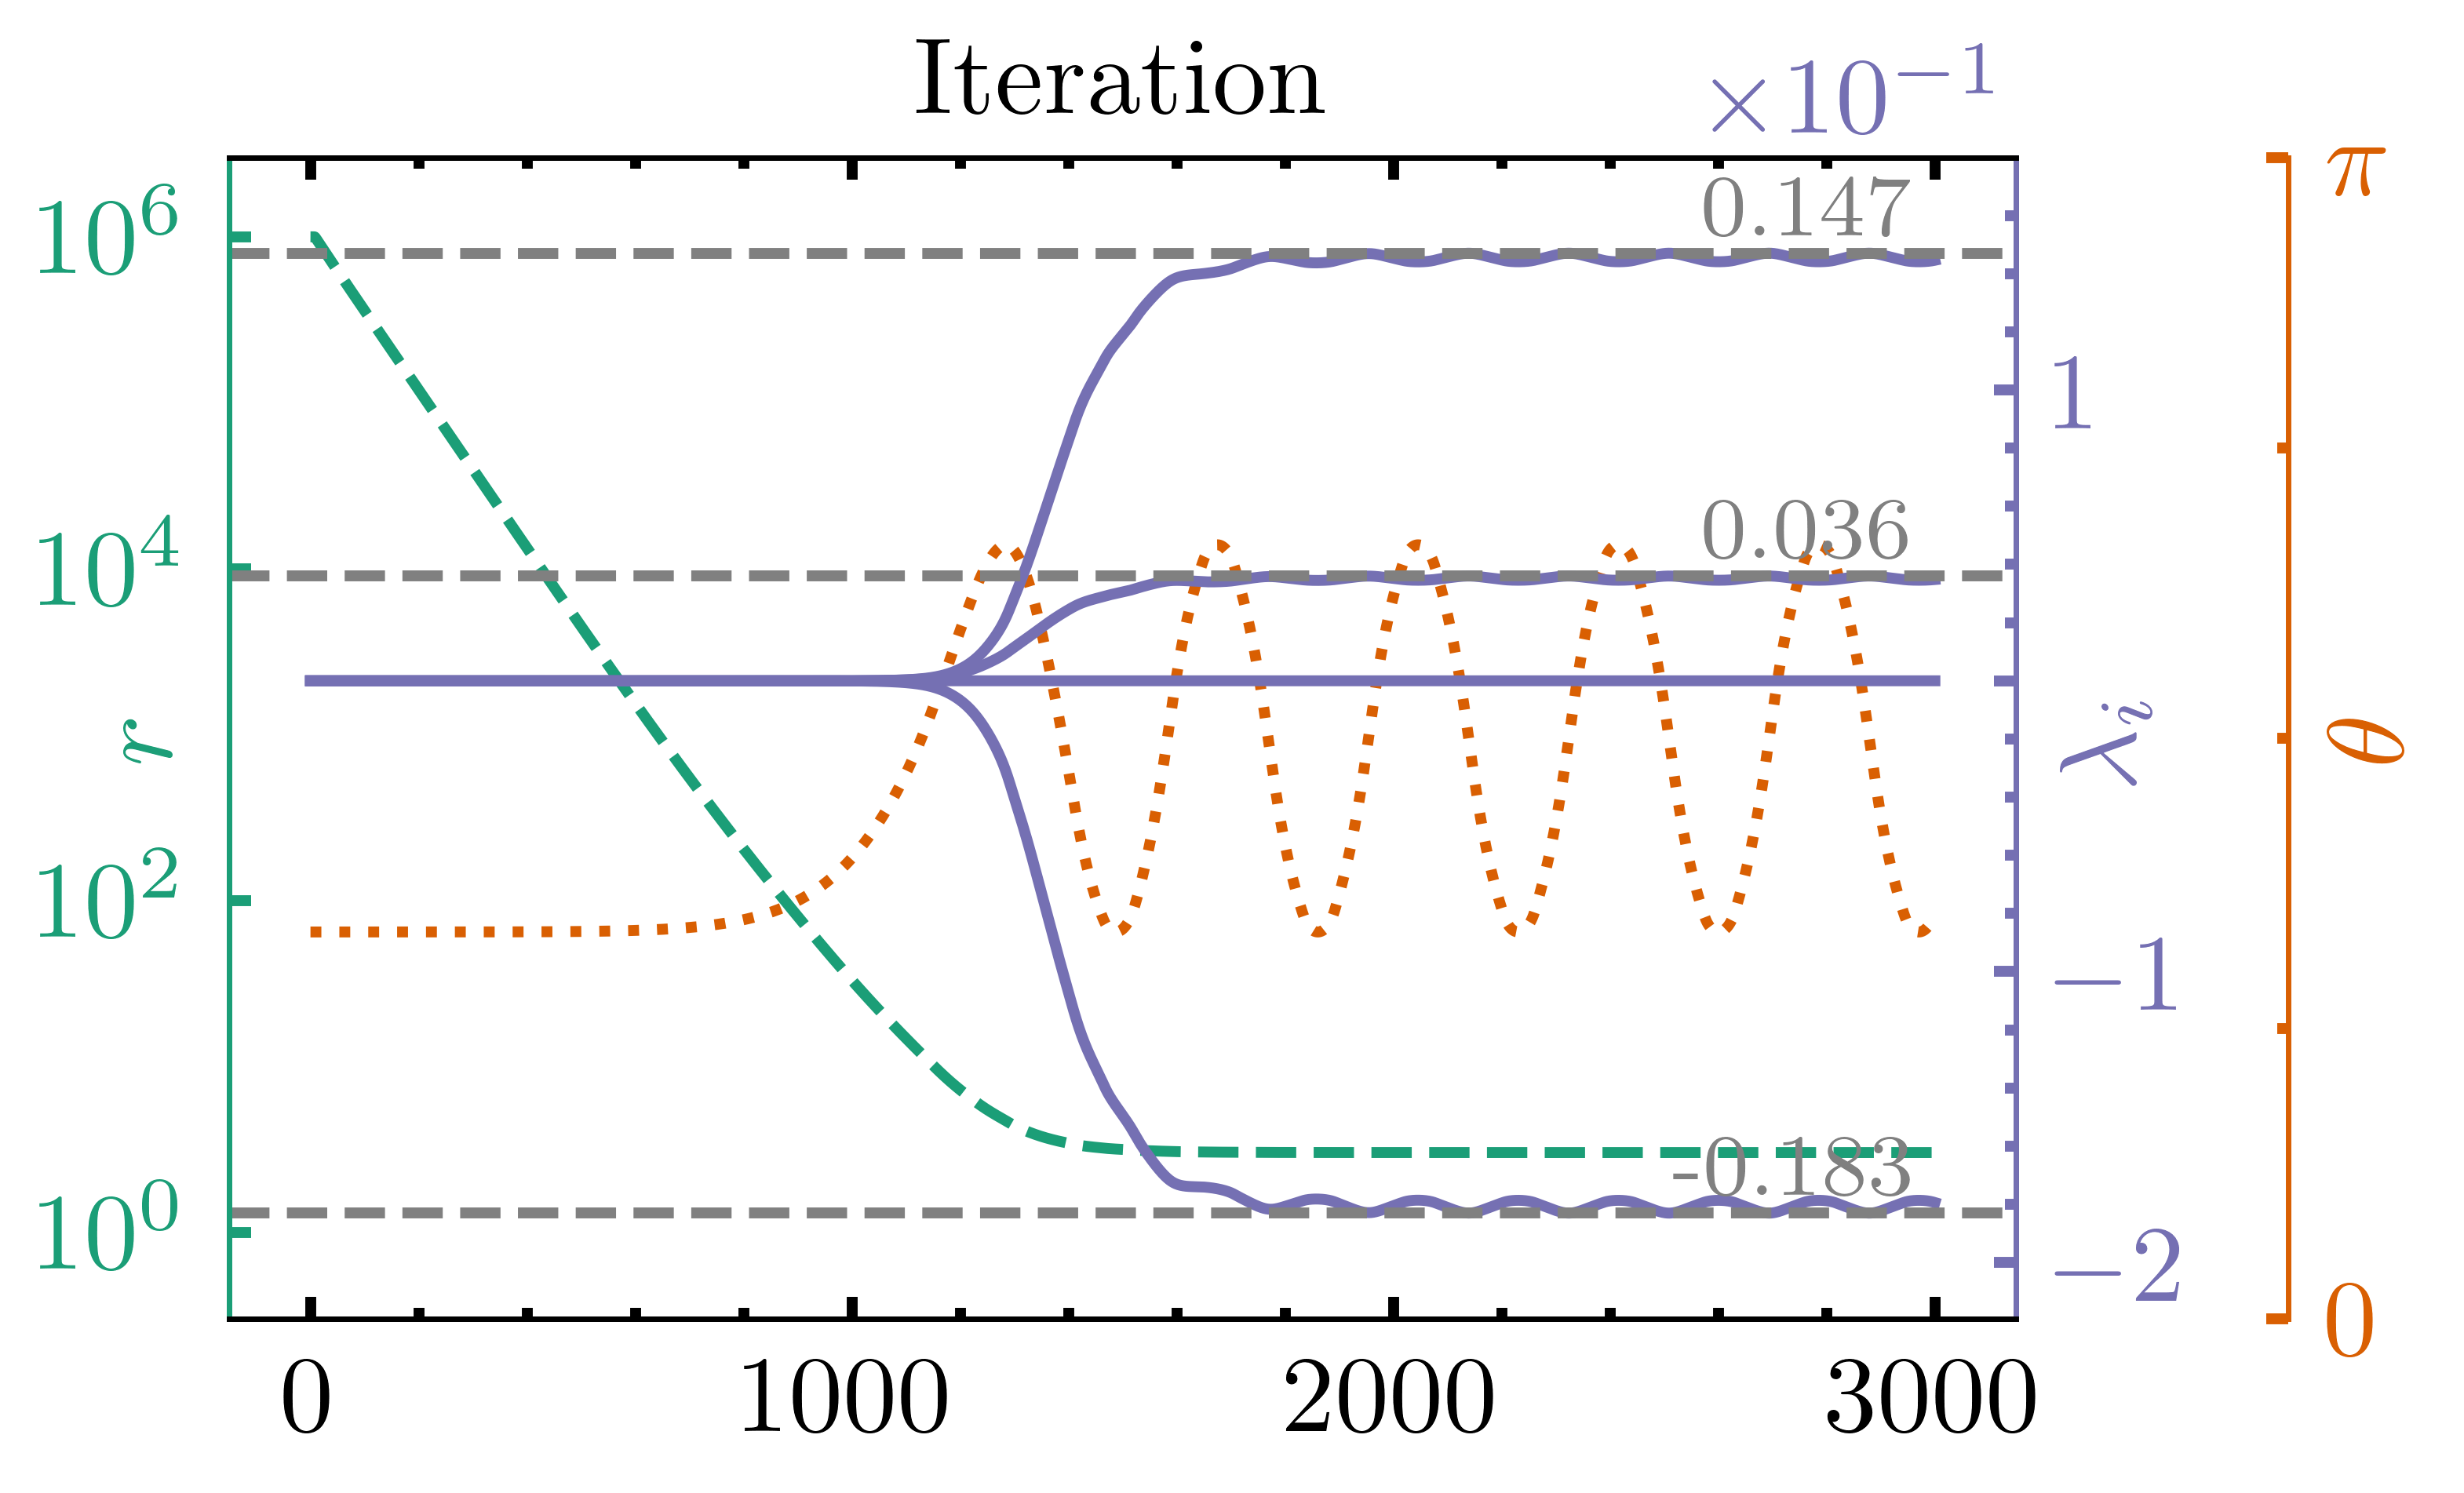
\includegraphics[width=\textwidth]{asset/eigensystem_a_0.50_Q_0.00_lambda_0.50_pro.png}
        \caption{$\Lambda = 0.5$, $a = 0.98$, $Q = 0$}
    \end{subfigure}
    \begin{subfigure}[b]{\columnwidth}
        \centering
        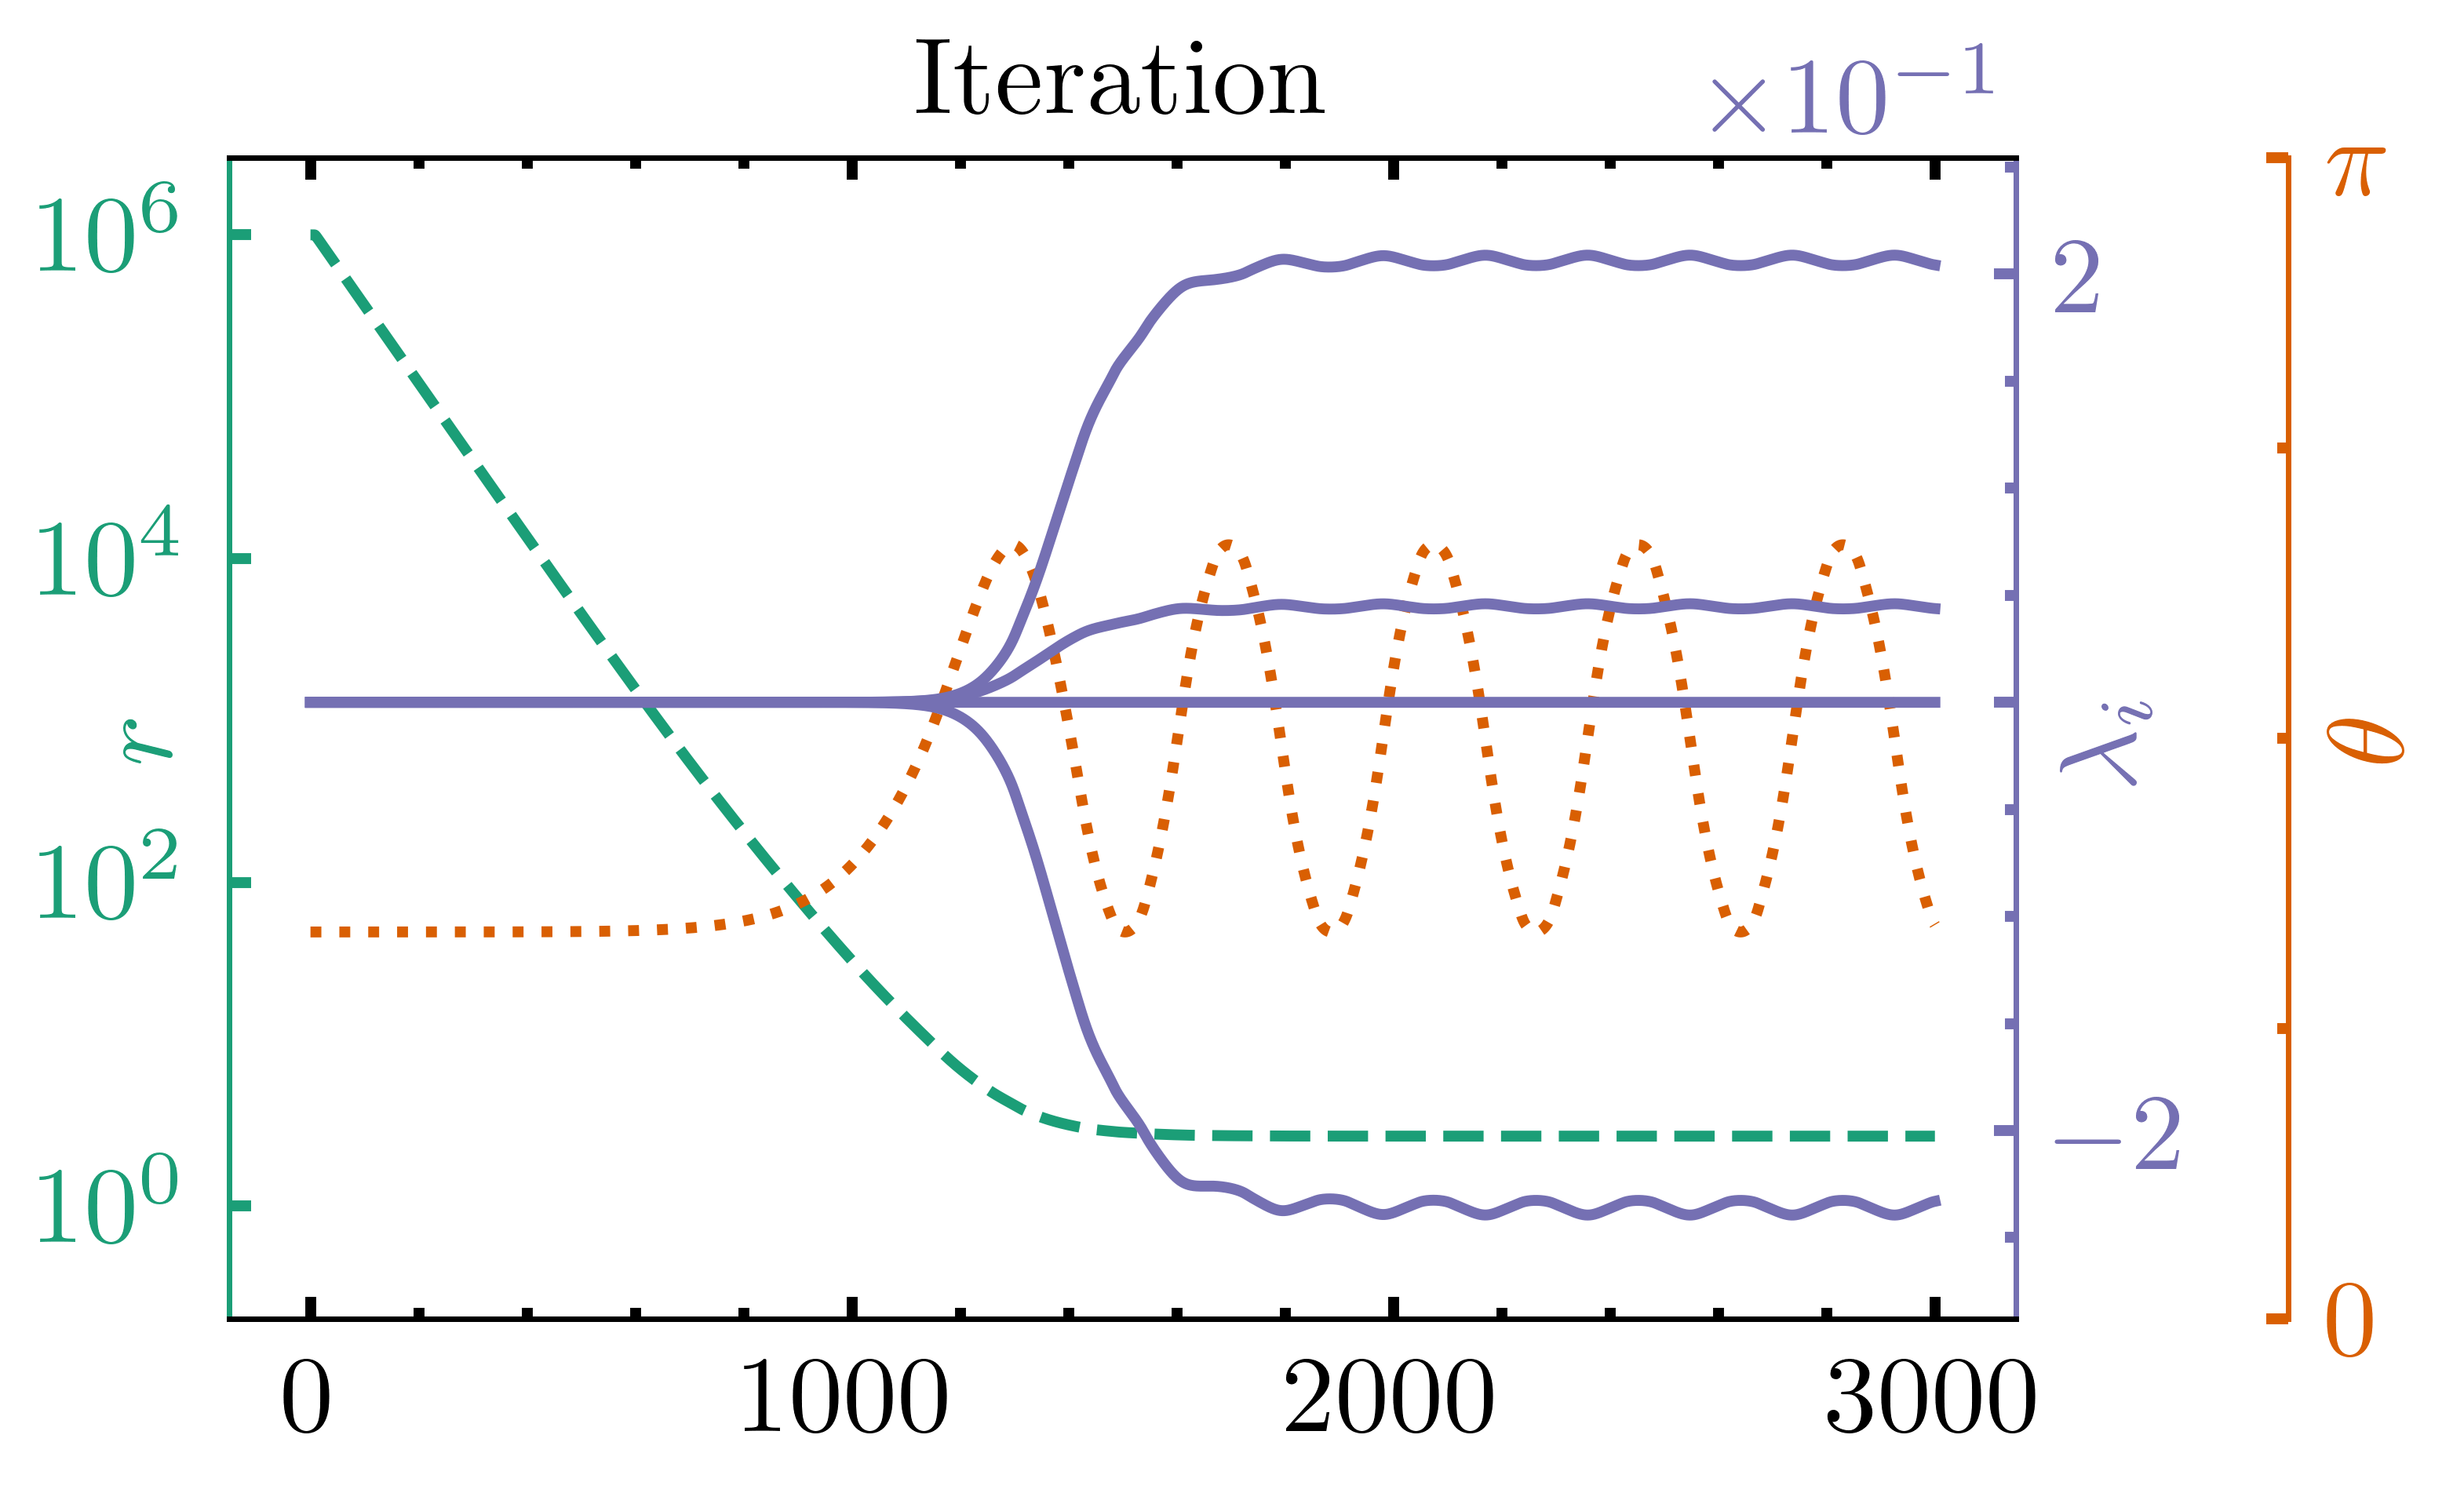
\includegraphics[width=\textwidth]{asset/eigensystem_a_0.50_Q_0.50_lambda_0.50_pro.png}
        \caption{$\Lambda = 0.5$, $a = 0.5$, $Q = 0.5$}
    \end{subfigure}
    \caption{Evolution of tidal eigenvalues along prograde IBSO geodesics in KN BH, with radial distance (green dashed), polar angle (orange dotted) and tidal eigenvalues (purple solid).}
    \label{fig:kn_simulations}
\end{figure}

In plots where $Q = 0$ (i.e. Kerr spacetime), we draw grey reference lines that represent the maximum tidal forces derived with a different analytical method \cite{Marck1983}. The excellent agreement suggests the correctness of the ZAMO approach in computing the tidal tensor.


%==========
\section{Conclusion} \label{sec:conclusion}
%==========


In this report, we have described the implementation of a general framework for deriving the local tidal tensor in any stationary, axisymmetric spacetime using the ZAMO frame. We use \texttt{Mathematica} for symbolic manipulation and \texttt{C++} for numerical integration. To the best of our knowledge, this is the first study that offers a general approach to computing the relativistic tidal forces along an arbitrary geodesic in a general spacetime. The flexibility of the approach allows both analytical and numerical studies of tidal forces in various spacetimes. It would be interesting to see if TDEs could serve as a different avenue for testing the validity of general relativity in the strong field regime, as has been done using X-ray spectroscopy and gravitational waves.

It is important to note that the ZAMO approach is not limited to IBSOs. One may choose any physically allowed initial conditions, integrate the geodesic equations and calculate the tidal forces along the trajectory. It may be of benefit to study the behaviour of the tidal forces for different geodesics drawn from a parameter space of initial conditions. This may provide insights into when and how TDEs occur and what properties of the BH we can infer from them. We hope that this report will be useful for future studies of TDEs and other relativistic phenomena related to tidal forces.

% Bibliography
\printbibliography


%==========
\appendix
\section{Conserved Quantities} \label{app:conserved}
%==========


A particle in Kerr-Newman spacetime has three conserved quantities:
\begin{equation}
    \begin{split}
        \epsilon &\equiv -p_{t} = g_{tt} \dot{t} + g_{t\phi} \dot{\phi} \, , \\
        l_{z} &\equiv p_{\phi} = g_{t\phi} \dot{t} + g_{\phi\phi} \dot{\phi} \, , \\
        q &\equiv p_{\theta}^{2} + \cos^{2}{\theta} \left[ a^{2} (\epsilon^{2} - 1) + \frac{l_{z}^{2}}{\sin^{2}{\theta}} \right]
    \end{split}
\end{equation}

The first two, energy and angular momentum, are conserved because spacetime is stationary and axisymmetric. The third Carter constant is due to the separability of the Hamilton-Jacobi equation in Kerr-Newman spacetime. We will further define another conserved quantity that measures the inclination angle of the particle's trajectory at spatial infinity:

\begin{equation}
    \sin{\iota} \equiv \frac{l_{z}}{\sqrt{l_{z}^{2} + q}} \, , \qquad \Lambda \equiv \cos{\iota} \, .
\end{equation}


%==========
\section{Innermost Bound Spherical Orbits} \label{app:ibso}
%==========


First integrals of the geodesic equations for neutral particles in Kerr-Newman spacetime are:
\begin{equation}
    \begin{split}
        \Sigma \frac{\mathrm{d}t}{\mathrm{d}\tau} &= -a(a \epsilon \sin^{2}{\theta} - l_{z}) + (r^{2} + a^{2}) \frac{T}{\Delta} \, , \\
        \Sigma^{2} \left( \frac{\mathrm{d}r}{\mathrm{d}\tau} \right)^{2} &= R \, , \\
        \Sigma^{2} \left( \frac{\mathrm{d}\theta}{\mathrm{d}\tau} \right)^{2} &= \Theta \, , \\
        \Sigma \frac{\mathrm{d}\phi}{\mathrm{d}\tau} &= -\left( a \epsilon - \frac{l_{z}}{\sin^{2}{\theta}} \right) + a \frac{T}{\Delta} \, ,
    \end{split}
\end{equation}
where:
\begin{equation}
    \begin{split}
        T(r) &\equiv \epsilon (r^{2} + a^{2}) - al_{z} \, , \\
        R(r) &\equiv T^{2} - \Delta (\mu_{m}^{2} r^{2} + k) \, , \\
        \Theta(\theta) &\equiv k - (l_{z} - a\epsilon)^{2} - \cos^{2}{\theta} \left[ a^{2} (\mu_{m}^{2} - \epsilon^{2}) + \frac{l_{z}^{2}}{\sin^{2}{\theta}} \right] \, ,
    \end{split}
\end{equation}
where $\mu_{m} = 1$ for massive particles with time-like geodesics and $\mu_{m} = 0$ for massless particles with null geodesics.

Innermost bound spherical orbits (IBSOs) are defined by the conditions $\epsilon = 1$ (innermost bound), $\mathrm{d}r/\mathrm{d}\tau = 0$ and $\mathrm{d}^{2}r/\mathrm{d}\tau^{2} = 0$ (spherical). That is, we require $R(\chi) = R'(\chi) = 0$. They give a condition on $l_{z}$:
\begin{equation}
    l_{z} = \frac{1}{a(\chi - 1)} \left[ \chi (\chi - Q^{2}) - a^{2} - \chi^{1/2} \Delta \right] \, ,
\end{equation}
and a characteristic equation for $\chi$:
\begin{equation} \label{eq:ibso_kn}
    \begin{split}
        0 &= 3\chi^{6} - (Q^{2} + 4) \chi^{5} + a^{2}(9\Lambda^{2} - 2) \chi^{4} \\
        &\quad+ a^{2} \left( 4 - 16\Lambda^{2} + 4Q^{2} - 6Q^{2}\Lambda^{2} + 3Q^{4}/a^{2} \right) \chi^{3} \\
        &\quad+ a^{2} \left( -a^{2} + 6a^{2} \Lambda^{2} \right) \chi^{2} \\
        &\quad- a^{2} Q^{2} \left( 4 + 16\Lambda^{2} - Q^{2} + Q^{2} \Lambda^{2} - Q^{4} \right) \chi^{2} \\
        &\quad+ a^{2} \left( a^{2} Q^{2} - 2a^{2} \Lambda^{2} Q^{2} + Q^{4} - 4Q^{4} \Lambda^{2} \right) \chi \\
        &\quad+ a^{6} \Lambda^{2} \\
        &\quad- 2 (2\chi - Q^{2})^{2} \chi^{3/2} (\chi^{2} - 2\chi + a^{2} + Q^{2}) \, .
    \end{split}
\end{equation}

It is straightforward to numerically solve the equation for $\chi$ and a corresponding $l_{z}$ given $a$, $Q$, and $\Lambda$. Solutions generally exist for both positive and negative $l_{z}$, corresponding to prograde and retrograde orbits respectively. For the same set of parameters and orbit direction, multiple solutions of $\chi$ may exist. The largest one is taken as the IBSO radius, as the particle cannot reach inner solutions.


%==========
\section{Local Tidal Tensor in Spherical Spacetime}
%==========


Assuming a general spherical metric described by Equation \ref{eq:spherical_metric} and setting $\theta = \pi/2$ and $\epsilon = 1$, the local tidal tensor can be written as:
\begin{equation}
    C =
    \begin{bmatrix}
        0 & 0         & 0         & 0         \\
        0 & C^{1}_{1} & 0         & C^{1}_{3} \\
        0 & 0         & C^{2}_{2} & 0         \\
        0 & C^{3}_{1} & 0         & C^{3}_{3}
    \end{bmatrix} \, ,
\end{equation}
where:
\begin{equation}
    \begin{split}
        f C^{1}_{1} &= 2 r^{3} A^{1/2} B \left( l_{z}^{2} + r^{2} \right) A'^{2} + r^5 B A'^{2} \\
        &\quad+ A^{2} r B' \left( \left( l_{z}^{2} + r^{2} \right)^{2} A'-2 l_{z}^{2} r \right) \\
        &\quad+ 2A^{2} B \left( l_{z}^{2} + r^{2} \right) \left( l_{z}^{2} A'-r \left( l_{z}^{2} + r^{2} \right) A'' \right) \\
        &\quad+ r A \left( A' \left( B \left( \left( l_{z}^{2} + r^{2} \right)^{2} A'-2 l_{z}^{2} r \right) + r^{4} B' \right) \right) \\
        &\quad-2 r^{5} A B A'' \\
        &\quad+ 2 r^{3} A^{3/2} \left( l_{z}^{2} + r^{2} \right) \left( A' B'-2 B A'' \right) \\
        &\quad-4 l_{z}^{2} r^{2} A^{5/2} B'-2 l_{z}^{2} r^{2} A^{3} B' \, ,
    \end{split}
\end{equation}
\begin{equation}
    \begin{split}
        (2 r^{4} A^{2} B^{2}) C^{2}_{2} &= B \left( r^3 \left( -A' \right)-2 l_{z}^{2} A^{2} (B-1) \right) \\
        &\quad+r A \left( A \left( l_{z}^{2}+r^{2} \right)-r^{2} \right) B' \, ,
    \end{split}
\end{equation}
\begin{equation}
    \begin{split}
        f C^{3}_{3} &= r A \left( A \left( l_{z}^{2}+r^{2} \right)-r^{2}\right) B' \left( 2 r ( A^{1/2} +1 )^{2}-l_{z}^{2} A'\right) \\
        &\quad+B \left( 2 l_{z}^{2} r A \left( A \left( l_{z}^{2}+r^{2} \right)-r^{2} \right) A'' \right) \\
        &\quad+B \left( l_{z}^{2} r \left( r^{2}-A \left( l_{z}^{2}+r^{2} \right) \right) A'^{2} \right) \\
        &\quad-2BA' \left( -l_{z}^{2} A+r^{2} A^{1/2} +r^{2} \right)^{2} \, ,
    \end{split}
\end{equation}
\begin{equation}
    \begin{split}
        &f \frac{A^{1/2}B^{1/2}}{l_{z} r} \left( \frac{B}{1/A - l_{z}^{2}/r^{2} - 1} \right)^{1/2} C^{1}_{3} = \\
        &- r A^{1/2} B A' \left( \left( l_{z}^{2} + r^{2} \right) A' - 2 r \right) \\
        &+ A^{3/2} \left( 2 B \left( r \left( l_{z}^{2} + r^{2} \right) A'' - l_{z}^{2} A' \right) \right) \\
        &- A^{3/2} r B' \left( \left( \left( l_{z}^{2} + r^{2} \right) A' - 2 r \right) \right)  \\
        &+ r^{2} A \left( 2 B \left( r A'' + A' \right) - r A' B' \right) + 2 r^{2} A^{5/2} B' \\
        &+ 4 r^{2} A^{2} B' - r^3 B A'^{2} \, ,
    \end{split}
\end{equation}
\begin{equation}
    C^{3}_{1} = C^{1}_{3} \, ,
\end{equation}
and:
\begin{equation}
    f(A, B) = 4 r^5 \left( A^{1/2} + 1 \right)^{2} A^{2} B^{2} \, .
\end{equation}

It is possible to relax the condition on $\theta$, $\epsilon$ and the angular parts of the metric. The latter is done by setting $g_{\theta\theta} = g_{\phi\phi}/\sin^{2}{\theta} = C(r)$. Explicit expressions for the local tidal tensor and its eigenvalues and eigenvectors can still be obtained. The expressions are too lengthy to be included here, but we invite the interested reader to use the accompanying \texttt{Mathematica} notebook to derive them. Our results are consistent with all of the cited papers in the notebook.


%==========
\section{Source Code} \label{app:code}
%==========


The source code is available at \href{https://unioxfordnexus-my.sharepoint.com/:f:/g/personal/exet5758_ox_ac_uk/EqVCppripCpAjYcxPht6mXABl-FsBaYHQBCxma3uGKZzXg?e=IZO2rz}{this link}. Note that Nexus365 login is required to access the files. The code is organised as follows:

\begin{itemize}
    \item \texttt{integrator\_unified} contains the \texttt{C++} source code for the integrator.
          \subitem Compile \texttt{main.cpp} to run the integrator.
          \subitem \texttt{analysis.ipynb} carries out plotting and analysis of the results using \texttt{Python}.
    \item \texttt{notebooks} contains the \texttt{Mathematica} notebooks for symbolic derivation.
          \subitem \texttt{tidal\_tensor\_newman.nb} derives the tidal tensor for Kerr-Newman spacetime.
          \subitem \texttt{tidal\_tensor\_spherical.nb} derives the tidal tensor for general spherical spacetimes and checks against various literature.
          \subitem \texttt{tidal\_tensor\_wormhole.nb} derives the tidal tensor for an exotic wormhole spacetime.
\end{itemize}



\end{document}